% Chapter 'Evaluation'

\section{Methods}
	\subsection{Hypothesis}
		There are many things we could evaluate, as both features, segmentation, and classification are critical parts of the application. Even if only evaluating on the classifier, the number of combinations of features, and parameters of features (window size and window skip), is huge. We want keep a single independent variable. To limit ourselves, we chose not to test any combinations of features, but rather single features one at a time. We will then test that feature for $K \in [1;10]$. We state the null hypothesis that two knn-classifiers with a different k and otherwise identical, will not have result in significantly different confusion tables.
		
		This will be tested for each feature and each feature configuration.
		We will test window sizes of 20ms, 10ms, and 5ms; and we will test window skips of 10ms, 5ms, 2ms respectively. This will be the case for all features using window: MFCC, Spectral Flux, Spectral Centroid, Spectral Skew, and Spectral Rolloff. Only the first 20 MFCC coefficients will be used. RMS and ZCR are calculated over the entire sound.
		
		To determine if the independent variable $k$ has any has any significant effect on resulting confusion tables, the chi squared test is used. The probability calculated will be divided with the number of test to correct it over many tests, also called the Bonferroni correction\citep{bonferroni}.
		Since we are testing over 10 different K, the amount of tests done in total will be $Tests = 10*9/2$.
		We have chosen that the null hypothesis can be disputed, if any calculated probability $p < alpha$, with $alpha=0.01$.
		
	\subsection{Measures}
		A confusion table is created for each test (each unique combination of variables). This will be shown in percentages (or rather, values between 0 and 1). Overall accuracy is calculated, along with precision, recall, and F-score for each class individually. For the sake of compactness, all the measures are included in an extended confusion table, as shown in the explanatory table \ref{table:eval:explanatory}. 
		The most important measure, for the sake of measuring our transcription system, would be the precision, that is, the amount of correctly transcribed sounds over the actual amount of that sound class.
		Recall should just be ignored, since we only test on the dataset, which means that we always test on all available samples of any given class, meaning that it would be the same as the amount of . This would be different, had the segmentation been part of the evaluation. It is included nonetheless, as further progress with this project might find a need for it. When looking at results, we will judge the performance primarily by accuracy, but secondarily by precision.

			\begin{table}
				\centering
				\begin{tabular}{|c | c | c | c | c |}
					\hline
				 & Real Class(1) & Real Class(2) & Real Class(3) & Precision\\ \hline
					Label(1)  & ... & ... & ... & ...\\ \hline
					Label(2)  & ... & ... & ... & ...\\ \hline
					Label(3) & ... & ... & ... & ...\\ \hline
					F-Score & ... & ... & ... & Accuracy \\ \cline{1-4}
				\end{tabular}
				\caption{$K=1$}
				\label{table:eval:explanatory}
			\end{table}
		
		
	\subsection{Training and Test Sets}
		The dataset consists of sound segments, segmented based on the annotations. This means that our segmentation of sound (present in our application), will not be part of the evaluation.
		The training and test sets of sounds for the KNN classifier are randomly chosen from the same pool (the dataset). It is distributed between the training and test set in a 70\%/30\% ratio, accordingly, for each class. This means there will not be a fixed number of sounds for each class (neither total nor divided), but rather a fixed distribution between the number of training and test sounds for each class. We can do this instead of e.g. k-fold cross validation, due to scale of our collected dataset. The ratio was suggested by our supervisor\footnote{Bob L. Sturm}. The composition of the entire dataset has been summarized in table \ref{table:eval:datasetComposition}. 
		Furthermore, all sounds with a duration less than the windowsize used for feature calculation, are removed before testing. This is done before splitting the dataset, such as to make sure we do not distort the 70/30 distribution.

		\begin{table}
			\centering
			\begin{tabular}{|l|r|r|}
					\hline
					Value  &  Count  & Percent \\ \hline
			      noise    &  150    & 10.19\% \\ \hline
			          k    &  466    & 31.66\% \\ \hline
			  undefined    &  130    &  8.83\% \\ \hline
			          s    &  331    & 22.49\% \\ \hline
			         hh    &  395    & 26.83\% \\ \hline
			      TOTAL    &  1472	 & 100.00\% \\ \hline

			\end{tabular}
			\caption{Dataset composition}
			\label{table:eval:datasetComposition}
		\end{table}
		
		
	\subsection{Test Implementation}		% REFERENCES TO APPENDIX!
		To ease the testing of the transcription system, some additional scripts were created: \texttt{prettyPrintTables.m}, \texttt{testPlots.m}, \texttt{printDataStats.m}, and \texttt{DoEverything.m}.
		The \texttt{printPrettyTables.m} script simply runs a test and formats the results in tables usable for \LaTeX, while \texttt{testPlots.m} creates plots for precision, recall, and F over K, including the overall accuracy in all three plots, and saves them as PNG images\footnote{\url{using: https://github.com/ojwoodford/export\_fig}}. They will not be described further, as they have no real functional effect on the system -  they are just helping facilitating the tests. These scripts are quite simple and well-commented, and thus should require no more than than a simple mention, as they do not include features, not already explained in chapter \ref{chapter:OurApproach}.
			
 
\section{Results}
	
	For all results found, some interpretation of the data and statistics will be presented, although it will be kept short due to the breadth of configurations tested. Further discussion about the relevance of the data, possible mistakes that affected results, or similar, will be covered in chapter \ref{chapter:Discussion}. Only the relevant results will be shown and discussed, based on the accuracy, however the other measures will be considered as well. All data can be found in appendix \ref{app:res}. 

	%
	% RMS
	%
	
	\subsection{Root Mean Square}
		\begin{figure}
		
			\centering\includegraphics[width=0.3\textwidth]{tex/appendices/test/rms11FP.png}
			\centering\includegraphics[width=0.3\textwidth]{tex/appendices/test/rms11_P.png}
			\centering\includegraphics[width=0.3\textwidth]{tex/appendices/test/rms11_R.png}
			
			\label{fig:eval:rms}
			\caption{Plots over K for Root Mean Square}
		\end{figure}

		\begin{table}
			\begin{subtable}[tbp]{0.45\textwidth}
				\centering
				\begin{tabular}{|c|c|c|c"c|}
					\cline{2-5}
				 \multicolumn{1}{c|}{} & \textbf{k}  & \textbf{s}  & \textbf{hh}  & Prec.\\ \hline
				 \textbf{s} & \textcolor{red}{0.719} & 0.212 & 0.161 & 0.714\\ \hline
				 \textbf{k} & 0.094 & \textcolor{red}{0.364} & 0.364 & 0.391\\ \hline
				 \textbf{hh} & 0.094 & 0.424 & \textcolor{red}{0.475} & 0.452\\ \Xhline{2\arrayrulewidth}
				 F & 0.717 & 0.377 & 0.463 & \textcolor{blue}{0.539}\\ \hline
				\end{tabular}
				\label{table:eval:rmsWorst}
				\caption{$K=1$ (Worst)}
			\end{subtable}
			
			\begin{subtable}[tbp]{0.45\textwidth}
				\centering
				\begin{tabular}{|c|c|c|c"c|}
					\cline{2-5}
				 \multicolumn{1}{c|}{} & \textbf{k}  & \textbf{s}  & \textbf{hh}  & Prec.\\ \hline
				 \textbf{s} & \textcolor{red}{0.791} & 0.141 & 0.059 & 0.840\\ \hline
				 \textbf{k} & 0.079 & \textcolor{red}{0.384} & 0.339 & 0.427\\ \hline
				 \textbf{hh} & 0.079 & 0.475 & \textcolor{red}{0.602} & 0.522\\ \Xhline{2\arrayrulewidth}
				 F & 0.815 & 0.404 & 0.559 & \textcolor{blue}{0.615}\\ \hline
				\end{tabular}
				\label{table:eval:rmsBest}
				\caption{$K=9$ (Best)}
			\end{subtable}
				
			\caption{Measures over K using RMS}
		\end{table}
	
		The best results using the RMS feature vector was observed using $K=9$, see table \ref{table:eval:rmsBest}. Some configurations had slightly higher precision in classes 's' and 'hh', although this seems minimal (see e.g. appendix  \ref{app:rms:k6} and \ref{app:rms:k8}). The worst observed was using $K=1$, see table \ref{table:eval:rmsWorst}. All tests performed using RMS, returned $p < alpha$, making the results significant, and disproving the null-hypothesis. All results from for the RMS feature can be found in appendix \ref{app:res:rms}.
		
	%
	%	ZCR
	%
	
	\subsection{Zero Crossing Rate}
		\begin{figure}
			\centering\includegraphics[width=0.3\textwidth]{tex/appendices/test/zcr11FP.png}
			\centering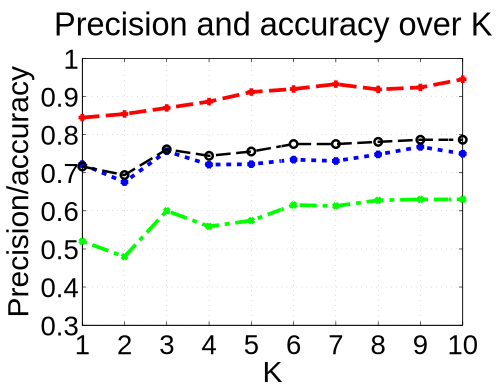
\includegraphics[width=0.3\textwidth]{tex/appendices/test/zcr11_P.png}
			\centering\includegraphics[width=0.3\textwidth]{tex/appendices/test/zcr11_R.png}
			\label{fig:eval:zcr}
			\caption{Plots over K for Zero Crossing Rate}
		\end{figure}
		
		\begin{table}
			\begin{subtable}[tbp]{0.45\textwidth}
				\centering
				\begin{tabular}{|c|c|c|c"c|}
					\cline{2-5}
					 \multicolumn{1}{c|}{} & \textbf{k}  & \textbf{s}  & \textbf{hh}  & Prec.\\ \hline
					 \textbf{s} & \textcolor{red}{0.871} & 0.081 & 0.017 & 0.924\\ \hline
					 \textbf{k} & 0.122 & \textcolor{red}{0.636} & 0.169 & 0.630\\ \hline
					 \textbf{hh} & 0.122 & 0.283 & \textcolor{red}{0.814} & 0.768\\ \Xhline{2\arrayrulewidth}
					 F & 0.896 & 0.633 & 0.790 & \textcolor{blue}{0.787}\\ \hline
				\end{tabular}
				\label{table:eval:zcrBest1}
				\caption{$K=9$ (Best)}
			\end{subtable}
		
			\begin{subtable}[tbp]{0.45\textwidth}
				\centering
				\begin{tabular}{|c|c|c|c"c|}
					\cline{2-5}
					 \multicolumn{1}{c|}{} & \textbf{k}  & \textbf{s}  & \textbf{hh}  & Prec.\\ \hline
					 \textbf{s} & \textcolor{red}{0.871} & 0.051 & 0.017 & 0.945\\ \hline
					 \textbf{k} & 0.122 & \textcolor{red}{0.636} & 0.169 & 0.630\\ \hline
					 \textbf{hh} & 0.122 & 0.313 & \textcolor{red}{0.814} & 0.750\\ \Xhline{2\arrayrulewidth}
					 F & 0.906 & 0.633 & 0.780 & \textcolor{blue}{0.787}\\ \hline
				\end{tabular}
				\label{table:eval:zcrBest2}
				\caption{$K=10$ (Best)}
			\end{subtable}
			
			\begin{subtable}[tbp]{0.45\textwidth}
				\centering
				\begin{tabular}{|c|c|c|c"c|}
					\cline{2-5}
					 \multicolumn{1}{c|}{} & \textbf{k}  & \textbf{s}  & \textbf{hh}  & Prec.\\ \hline
					 \textbf{s} & \textcolor{red}{0.885} & 0.162 & 0.042 & 0.854\\ \hline
					 \textbf{k} & 0.108 & \textcolor{red}{0.475} & 0.305 & 0.480\\ \hline
					 \textbf{hh} & 0.108 & 0.364 & \textcolor{red}{0.653} & 0.675\\ \Xhline{2\arrayrulewidth}
					 F & 0.869 & 0.477 & 0.664 & \textcolor{blue}{0.694}\\ \hline
				\end{tabular}
				\label{table:eval:zcrWorst}
				\caption{$K=2$ (Worst)}
			\end{subtable}
			
			\caption{Measures over K using ZCR}
		\end{table}
		
		The best results using ZCR was a tie $K=9$ (table \ref{table:eval:zcrBest1}) and $k=10$ (\ref{table:eval:zcrBest2}). In the results from $K=9$, the precision of the hh is slightly better than in $K=10$. In $K=10$, the precision of the kick is slightly better.
		Th worst results was observed with $K=2$ (table \ref{table:eval:zcrWorst}). As with our results using RMS, we found that all probabilities were significant.
		
	%	
	%	MFCC
	%	
		
	\subsection{Mel Frequency Cepstrum Coefficients}
		\begin{figure}
			\centering\includegraphics[width=0.3\textwidth]{tex/appendices/test/mfcc2010FP.png}
			\centering\includegraphics[width=0.3\textwidth]{tex/appendices/test/mfcc2010_P.png}
			\centering\includegraphics[width=0.3\textwidth]{tex/appendices/test/mfcc2010_R.png}
			
			\caption{Plots over K for MFCC with 20ms windows and 10ms window skips}
		\end{figure}
		\begin{figure}
			\centering\includegraphics[width=0.3\textwidth]{tex/appendices/test/mfcc105FP.png}
			\centering\includegraphics[width=0.3\textwidth]{tex/appendices/test/mfcc105_P.png}
			\centering\includegraphics[width=0.3\textwidth]{tex/appendices/test/mfcc105_R.png}
			
			\caption{Plots over K for MFCC with 10ms windows and 5ms window skips}
		\end{figure}
		\begin{figure}
			\centering\includegraphics[width=0.3\textwidth]{tex/appendices/test/mfcc52FP.png}
			\centering\includegraphics[width=0.3\textwidth]{tex/appendices/test/mfcc52_P.png}
			\centering\includegraphics[width=0.3\textwidth]{tex/appendices/test/mfcc52_R.png}
			
			\caption{Plots over K for MFCC with 5ms windows and 2ms window skips}
		\end{figure}\clearpage
		
		Over all three configurations of the MFCC feature vector, the best performing were $K=7$ and $K=8$, when using a window size of 5ms and skip of 2ms, see table \ref{table:eval:mfccBest1} and \ref{table:eval:mfccBest2}. Although some of other results with the same parameters reach similar performance in regards to precision per class (see appendix \ref{tlmfcc52}). The worst performing, by accuracy, is using 20ms window size and 10ms skip with $K=2$ (see table \ref{table:eval:mfccWorst}). It still has better precision for kick than some others(e.g. $K=4$ or $K=6$), but some have similar hh precision (e.g. $K=1$ or $K=6$). All configurations, both in parameters and K, disproved the null hypothesis with $alpha=0.01$.
		
		
	%
	% SC
	%
	\subsection{Spectral Centroid}
		\begin{figure}
			\centering\includegraphics[width=0.3\textwidth]{tex/appendices/test/scentroid2010FP.png}
			\centering\includegraphics[width=0.3\textwidth]{tex/appendices/test/scentroid2010_P.png}
			\centering\includegraphics[width=0.3\textwidth]{tex/appendices/test/scentroid2010_R.png}
			
			\caption{Plots over K for Spectral Centroid with 20ms windows and 10ms window skips}
		\end{figure}
		\begin{figure}
			\centering\includegraphics[width=0.3\textwidth]{tex/appendices/test/scentroid105FP.png}
			\centering\includegraphics[width=0.3\textwidth]{tex/appendices/test/scentroid105_P.png}
			\centering\includegraphics[width=0.3\textwidth]{tex/appendices/test/scentroid105_R.png}
				
				\caption{Plots over K for Spectral Centroid with 10ms windows and 5ms window skips}
		\end{figure}
		\begin{figure}
			\centering\includegraphics[width=0.3\textwidth]{tex/appendices/test/scentroid52FP.png}
			\centering\includegraphics[width=0.3\textwidth]{tex/appendices/test/scentroid52_P.png}
			\centering\includegraphics[width=0.3\textwidth]{tex/appendices/test/scentroid52_R.png}
				
				\caption{Plots over K for Spectral Centroid with 5ms windows and 2ms window skips}
		\end{figure}\clearpage
		
		% BEST: 9(10,5)
		% WORST: 2
		% CHI: All significant
		The best configuration found was 10ms windows and 5ms window skips, with $K=9$, as shown in table \ref{table:eval:centroidBest}. Some results show similar or better precision in some classes, e.g. $K=8$, seen in table \ref{table:eval:centroidSimilar}. The worst result seen was using 20ms window size, 10ms window skip, as shown in table \ref{table:eval:centroidWorst}.
		Once again, every single test done, is deemed significant on the grounds of $alpha=0.01$.
		
				
	% 
	% SS
	%
	\subsection{Spectral Skew}
			
		\begin{figure}
			\centering\includegraphics[width=0.3\textwidth]{tex/appendices/test/sskew2010FP.png}
			\centering\includegraphics[width=0.3\textwidth]{tex/appendices/test/sskew2010_P.png}
			\centering\includegraphics[width=0.3\textwidth]{tex/appendices/test/sskew2010_R.png}
			
			\caption{Plots over K for Spectral Skew with 20ms windows and 10ms window skips}
		\end{figure}
		
		\begin{figure}
			\centering\includegraphics[width=0.3\textwidth]{tex/appendices/test/sskew105FP.png}
			\centering\includegraphics[width=0.3\textwidth]{tex/appendices/test/sskew105_P.png}
			\centering\includegraphics[width=0.3\textwidth]{tex/appendices/test/sskew105_R.png}
				
				\caption{Plots over K for Spectral Skew with 10ms windows and 5ms window skips}
		\end{figure}
		\begin{figure}
			\centering\includegraphics[width=0.3\textwidth]{tex/appendices/test/sskew52FP.png}
			\centering\includegraphics[width=0.3\textwidth]{tex/appendices/test/sskew52_P.png}
			\centering\includegraphics[width=0.3\textwidth]{tex/appendices/test/sskew52_R.png}
				
				\caption{Plots over K for Spectral Skew with 5ms windows and 2ms window skips}
		\end{figure}\clearpage
		
		% BEST: 5ms 2ms, K=5, best k, best s, these have better hh (10ms5ms, K)
		% WORST: 20ms 10ms2 K=2. Some (same parameters, K=1, K=3, K=6) har slightly lower precision with kicks.
	
	%
	% SF
	%
	\subsection{Spectral Flux}
		
		\begin{figure}
		
		
			\centering\includegraphics[width=0.3\textwidth]{tex/appendices/test/sflux2010FP.png}
			\centering\includegraphics[width=0.3\textwidth]{tex/appendices/test/sflux2010_P.png}
			\centering\includegraphics[width=0.3\textwidth]{tex/appendices/test/sflux2010_R.png}
			
			\caption{Plots over K for Spectral Flux with 20ms windows and 10ms window skips}
		\end{figure}
		\begin{figure}
		
		
			\centering\includegraphics[width=0.3\textwidth]{tex/appendices/test/sflux105FP.png}
			\centering\includegraphics[width=0.3\textwidth]{tex/appendices/test/sflux105_P.png}
			\centering\includegraphics[width=0.3\textwidth]{tex/appendices/test/sflux105_R.png}
				
				\caption{Plots over K for Spectral Flux with 10ms windows and 5ms window skips}
		\end{figure}
		\begin{figure}
		
		
			\centering\includegraphics[width=0.3\textwidth]{tex/appendices/test/sflux52FP.png}
			\centering\includegraphics[width=0.3\textwidth]{tex/appendices/test/sflux52_P.png}
			\centering\includegraphics[width=0.3\textwidth]{tex/appendices/test/sflux52_R.png}
				
				\caption{Plots over K for Spectral Flux with 5ms windows and 2ms window skips}
		\end{figure}
		
	% BEST:
	% WORST:

